\section{Projekt Valhalla}\label{sec:valhalla}

Das OpenJDK-Projekt \emph{Valhalla}~\cite{openjdk-valhalla} besteht aus drei wesentlichen Neuerungen, die in folgenden \acp{jep} definiert sind:

\begin{itemize}
    \item \ac{jep} 169: Value Objects~\cite{jep-169}
    \item \ac{jep} 193: Variable Handles~\cite{jep-193}
    \item \ac{jep} 218: Generics over Primitive Types~\cite{jep-218}
\end{itemize}

Grundlage für die Änderungen des Projekts stellen die \emph{Value Objects} dar.
Deren Ziel ist es, die \ac{jvm} mit Unterstützung für neue benutzerdefinierbare Typen zu erweitern, die im Vergleich zu bestehenden Klassen keine Referenzsemantik haben, sondern sich wie primitive Datentypen verhalten.
\ac{jep} 169 selber beschäftigt sich nur mit einer kleinen Erweiterung der JVM in diese Richtung.
Unterabschnitt~\ref{subsec:value-types} betrachtet das Ziel der Value Types als Ganzes.

Die \emph{Variable Handles} bezeichnen einen Teil der Java Standard-Bibliothek, die präziseren Zugriff auf Felder von Objekten und Array-Elementen ermöglichen.
Die Implementierung der API erfolgte bereits in Java 9 und wird daher nicht näher in dieser Arbeit betrachtet.

Die Erweiterung von generischen Typen mit Unterstützung für primitive Typen ist der größte Teil des Projekts.
Sie verlangt weitreichende Änderungen, die sowohl die Sprache als auch die \ac{jvm} betreffen.
In Unterabschnitt~\ref{subsec:primitive-generics} erfolgt eine Vertiefung in dieses Thema.

\subsection{Value Types}\label{subsec:value-types}

Seit der ersten Version von Java im Jahr 1995 verfolgt die Programmiersprache den Ansatz, dass alles außer primitive Werte ein Objekt ist.
Das unterscheided Java von Programmiersprachen wie C oder C++, wo primitive Werte sowie durch Klassen und Structs definierte Aggregate davon zunächst nur einfache Werte sind und erst durch Pointer eine Referenzsemantik erhalten.

In Java sind hingegen alle Variablen und Parameter vom Typ einer Klasse implizit Pointer.
Dies vereinfacht das Programmiermodell und ist weniger fehleranfällig, besonders durch die Präsenz des Garbage Collectors.
Es führt jedoch auch dazu, dass alle Zugriffe auf Daten in diesen Objekten über Indirektion erfolgen.
Dies verringert die Lokalität der Daten und führt auf heutiger Hardware, auf der Zugriffe auf den Hauptspeicher wesentlich länger dauern als auf den CPU-Cache-Speicher, zu deutlich langsamerer Performance. % TODO ww führt
Weiterhin erzeugen Referenzen einen deutlichen höheren Speicherverbrauch, wie ein Beispiel zeigen wird. % TODO wo?
Zuletzt sorgt die Allokation und Freigabe des Speichers, besonders bei einer Vielzahl kleiner Objekte, für einen Verwaltungsaufwand seitens des Allocators und Garbage Collectors.

Aufgrund dieser Performance-\ und Speicherbedenken suchen viele Java-Entwickler nach Möglichkeiten, Klassen und Objekte zu umgehen.
Meist entsteht dabei Code, der händische Optimierungen auf Kosten von Lesbarkeit, Abstraktion und Fehlersicherheit enthält.
Value Types sollen dies vermeiden.

% Unterschiede zu Referenzen, Pointerfreiheit
Es soll nun betrachtet werden, was Value Types von regulären Referenztypen unterscheided.
Größter Unterschied ist die \emph{Pointerfreiheit}.
Ohne Pointer funktionieren einige Konzepte nicht mehr, die bisher alltäglich waren.
So besitzen Werte keine Identität mehr, die verglichen werden könnte, und damit auch keinen Identitäts-Hashcode.
Weiterhin können sie nicht mehr als Monitor dienen, da ohnehin nicht von zwei Threads darauf zugegriffen werden kann.
Die \code{clone}-Operation ist nicht mehr sinnvoll, ebenso der Finalizer, da die Werte nicht mehr vom Garbage Collector verarbeitet werden.
Auch \code{null} ist kein gültiger Wert mehr, allerdings wäre eine Alternative möglich, die den Speicher für den Wert auf null setzt.
Zuletzt kann nicht von Value Types geerbt werden, da im Voraus bekannt sein muss, wie viel Speicherplatz reserviert werden muss, was mit Vererbung nicht statisch entschieden werden könnte.
Veränderungen der Felder von Werten würde sich nur auf die lokale Kopie auswirken, wie es bereits von primitiven Typen bekannt ist.
Die Veränderung von \code{this} in Methoden eines Value Types ist folglich nicht mehr sinnvoll, wodurch Seiteneffekte vermieden werden und nachvollziehbarer Code entsteht.

% Value-basierte Klassen
Seit Java 8 definiert die Sprache bereits ein Konzept, das den Value Types ähnelt: die Value-basierten Klassen~\cite{value-based-classes}.
Dabei handelt es sich um eine Konvention, an die von einigen Klassen der Standardbibliothek eingehalten wird und auch für Bibliotheksautoren und andere Endbenutzer der Sprache verfügbar ist.
Wesentlich bei Value-basierten Klassen ist der Einsatz von Feldern, die \code{final} sind, wodurch Instanzen dieser Klassen unveränderbar werden.
Weiterhin dürfen diese Klassen keinen öffentlich zugänglichen Konstruktor besitzen, sondern müssen stets über eine Factory-Methode instanziiert werden.
Dadurch gegen sie keine Garantien über die Identität erstellter Objekte.
Die Factory-Methode kann beispielsweise ihre Rückgabewerte in einem Cache speichern.
Aufgrund der fehlenden Identität ist es nicht sinnvoll, Identitätsvergleiche mit \code{==} durchzuführen.
Folglich müssen stets \code{equals} und \code{hashCode} implementiert werden.
Die Verwendung von Identitäts-basierten Operationen und Synchronisierung auf Value-basierten Klassen ist zwar derzeit nicht verboten, da es sich um eine Konvention handelt, kann aber zu unerwarteten Ergebnissen führen.
Somit erfüllen Value-basierte Klassen fast alle zuvor genannten Punkte zur Pointerfreiheit.
Ausnahme ist die Verwendung von \code{null} als erlaubter Wert sowie die Möglichkeit zur Vererbung.
Dies ist jedoch bei derzeitigen Beispielen für Value-basierte Klassen wie \code{java.lang.Integer} und \code{java.util.Optional} ohnehin nicht üblich.

% Inline Classes
Mit Projekt Valhalla soll die Konvention der Value-basierten Klassen nun Sprach- und \ac{jvm}-Unterstützung erhalten.
Diese trägt die Bezeichnung \emph{Inline-Klassen}~\cite{object-model}, die sich aus dem Schlüsselwort \code{inline} ableitet, das für die Deklaration von Value Types eingesetzt wird.
Listing~\ref{inline-class-example} zeigt, wie eine Inline-Klasse aussehen kann.
Dabei ist zu beachten, dass sich der Code nur durch das Schlüsselwort \code{inline} von einer regulären Klasse unterscheidet.
Nach dem Motto ``Codes like a class, works like an int''~\cite{object-model} sollen die syntaktischen Änderungen bewusst klein sein.

\begin{listing}
    \begin{minted}{java}
        inline class Point {
            private int x;
            private int y;

            public Point(int x, int y) {
                this.x = x;
                this.y = y;
            }

            public int x() { return x; }
            public int y() { return y; }
        }
    \end{minted}
    \caption{Beispiel für eine Inline-Klasse (aus~\cite{object-model})}
    \label{inline-class-example}
\end{listing}

% Primitive untergeordnet
Mit der Einführung von Inline-Klassen wird die Unterscheidung zwischen primitiven und Referenz-Typen abgeschafft.
Nun wird zwischen Inline- und Referenz-Typen unterschieden;
die primitiven Typen werden den Inline-Typen untergeordnet.
% T.default
Weiterhin kann nun für alle Typen ein Default-Wert definiert werden, der mit \code{T.default} bezeichnet wird.
Für primitive Typen bleibt dieser \code{0} oder \code{false}, während Referenztypen \code{null} erlauben.
Inline-Typen definieren ihren Default-Wert als eine Instanz, bei der alle Felder mit dem jeweiligen Default-Wert belegt sind.

% Marker interfaces
Unter Umständen kann es nützlich sein, zur Laufzeit zu ermitteln, ob es sich bei einem Wert um eine Referenz oder einen Inline-Wert handelt.
Dafür werden neue Interfaces eingeführt, von denen automatisch und implizit alle Klassen erben:
\code{IdentityObject} für Referenzen und \code{InlineObject} für Inline-Klassen.
So kann entschieden werden, ob Identitätsoperationen wie \code{==} oder Synchronisierung sinnvoll sind.
% Interfaces + Klassenvererbung
Inline-Klassen dürfen auch von regulären Interfaces erben.
Ebenfalls soll es möglich sein, sie von Klassen erben zu lassen, solange diese nicht den Anforderungen an Inline-Klassen widersprechen.
Nicht erlaubt wären beispielsweise Superklassen mit nicht-finalen Feldern oder Methoden, die \code{synchronized} sind.
Ein Beispiel für eine solche Klasse ist \code{Object}, von dem weiterhin alle Klassen erben.

% Boxing
Mit der Unterordnung von primitiven Typen werden auch diese ohne Boxing von \code{Object} erben.
Boxing wird dann zu einer Operation, die von der JVM intern durchgeführt wird und nicht mehr nur durch den Compiler implementierter syntaktischer Zucker ist.
% Arrays
Das hat zur Folge, dass Array-Typen anders voneinander erben.
Insbesondere kann nun ein \code{int[]} direkt in ein \code{Integer[]} oder ein \code{Object[]} umgewandelt werden.
Ein ähnliches Verhalten zeigen die benutzerdefinierten Inline-Klassen.
% Referenz-Wrapper T.ref
Anders als bei primitiven Typen gibt es jedoch dabei keine explizit definierten Referenz-Wrapper.
Stattdessen soll neue Syntax hinzugefügt werden, mit der Referenz-Wrapper für Inline-Klassen benannt werden können.
Diese nimmt die Form \code{T.ref} an, wobei \code{T} eine Inline-Klasse bezeichnet.
Im Gegensatz dazu steht die Form \code{T.val}, die explizit den Inline-Typ benennt.

% Memory example
Um das Speicherproblem näher zu erläutern, soll nun ein Beispiel betrachtet werden.
Es sollen einige ganzzahlige Punkte im zweidimensionalen Raum gespeichert die einen Pfad bilden.
Die Punkte sind als Objekte mit zwei \code{int}-Feldern modelliert, der Pfad als Array von Punkten.
Bei einer Pfadlänge von drei berechnet sich der Speicherverbrauch wie folgt:

\[ \SI{24}{\byte} \text{(Array-Header)} + 3 \cdot \SI{8}{\byte} \text{(Referenzen im Array)} + 3 \cdot (\SI{16}{\byte} \text{(Objekt-Header)} + 2 \cdot \SI{4}{\byte} \text{(int-Werte)}) = \SI{120}{\byte} \]

Ein Objekt, das zwei \code{int}-Werte beeinhaltet, benötigt auf einer 64-bit \ac{jvm} $\SI{8}{\byte}$ für die Referenz selber, $\SI{16}{\byte}$\footnote{Mit \code{-XX:+UseCompressedOops} könnte dies auf $\SI{12}{\byte}$ reduziert werden, allerdings kommen dann $\SI{4}{\byte}$ Padding hinzu, da die Größere von Objekten im Heap ein Vielfaches von $\SI{8}{\byte}$ sein muss.} für den Objekt-Header und je $\SI{4}{\byte}$ für die beiden \code{int}-Werte.
Die Größe eines Array-Headers beträgt $\SI{24}{\byte}$.
Mit drei Objekten ergibt sich also insgesamt ein Speicherverbrauch von $\SI{120}{\byte}$.

Das gleiche Beispiel soll nun mit Value-Typen realisiert werden.
Dabei entfallen die Objekt-Header und Referenzen vollständig.
Der neue Speicherverbrauch berechnet sich also wie folgt:

\[ \SI{24}{\byte} \text{(Array-Header)} + 3 \cdot 2 \cdot \SI{4}{\byte} \text{(int-Werte)} = \SI{48}{\byte} \]

Folglich konnten $\SI{72}{\byte}$ eingespart werden.
Zu beachten ist auch, dass die gesamten Daten des Arrays mit einer Größe von $\SI{48}{\byte}$ in eine Cache-Zeile passen, wenn bei deren Größe von $\SI{64}{\byte}$ ausgangen wird.
Der Effekt wird verstärkt, wenn das Array mehr Elemente enthält.

In Abbildung~\ref{fig:memory-usage} erfolgt eine grafische Darstellung des verringerten Speicherverbrauchs.
Sie zeigt links das Speicherlayout in heutigen \acp{jvm} und rechts das Speicherlayout, wenn Value Types für die Punkte verwendet werden.
Die Höhe der Rechtecke mit Zahlen entspricht hier $\SI{4}{\byte}$.

\begin{figure}
    \centering
    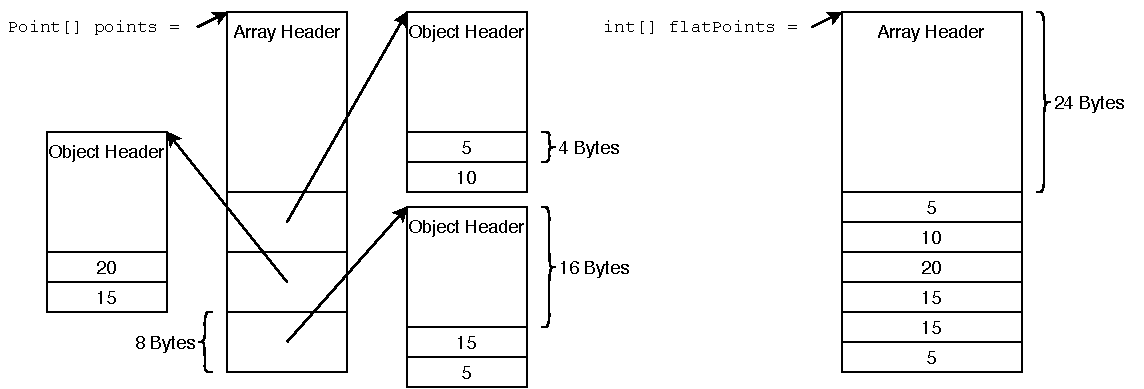
\includegraphics{img/memory-usage.pdf}
    \caption{Vergleich des Speicherlayouts eines Arrays von Punkten heute und mit Value Types}
    \label{fig:memory-usage}
\end{figure}

Die zweidimensionalen Punkte als Teil eines Pfades sind nur ein kleines, anwendungsspezifisches Beispiel.
Grundsätzlich lassen sich jedoch mit Value Types eine Vielzahl von neuen Datentypen definieren, die breite Anwendung finden können.
Dazu gehören im Bereich der numerischen Datenverarbeitung komplexe, vorzeichenlose und Dezimalzahlen, Binärzahlen größer als 64 bit und Vektoren, die auf modernen \acp{cpu} effizient verarbeitet werden können.
Auch algebraische Datentypen wie \code{Optional}, \code{Either}, \code{Unit} und Tupel sind wichtige Einsatzmöglichkeiten.
Letztere benötigen jedoch besondere Sprachunterstützung, die noch nicht Teil des Projekts ist.

\subsection{Primitive und generische Typen}\label{subsec:primitive-generics}
